\documentclass{MathematicaReport}

% PACKAGES
\usepackage{parskip}
\usepackage{mathtools}
\usepackage{float}
\usepackage{tikz}
\usetikzlibrary{patterns}

\place{Gliwice}
\date{\today}
\tasknumber{1}
\title{Comparative analysis of methods for approximating functions}
\author{Jakub Pietrasik, Bartosz Lewandowicz, Szymon Hankus}
\field{Informatics -- sem. V}


\begin{document}
\maketitle

\section{Project objective}
The goal of the project is to explain, present, and compare three methods of
approximating functions either from a set of given points or by approximating
the function itself. The methods that we chose are:
\begin{enumerate}
	\item Interpolation using Lagrange polynomials
	\item Fourier series
	\item The least squares method
\end{enumerate}

\section{Lagrange polynomials}
\textbf{Lagrange polynomials} are polynomials \( w(x) \) that interpolate a 
given set of points
\( P = \{ (x_0, y_0)\)\(,\ (x_1, y_1)\)\(,\ldots\) \(,\ (x_n, y_n) \} \)
Which means that they satisfy the following condition:

\[
	\forall_{(x_i, y_i) \in P}\ w(x_i) = y_i
\]

In other words, when a polynomial \textbf{interpolates} the dataset, it passes 
through all of the points in said dataset.
The Lagrange interpolating polynomial is the unique polynomial of lowest degree 
that interpolates a given set of data

Langrage polynomials for a given set of data are calculated using the following
formula
\[
	w(x) = \sum_{i=0}^n y_i \cdot \prod_{\begin{smallmatrix}0\le j\le n\\ j\neq i\end{smallmatrix}}
	 \frac{x-x_j}{x_i-x_j}
\]

In the next section, I would like to demonstrate how this formula can be
obtained and that it is actually quite straightforward and intuitive.

\subsection{How to arrive at the formula for Lagrange polynomials?}
This formula might seem daunting at first, but let us first consider a
polynomial \( w_i(x) \) that \textbf{goes through only one point \( (x_i, y_i) \) 
and is equal to 0 for the rest of the points}.

\begin{enumerate}
	\item For a given pair \( (x_i, y_i) \), it has to be equal to \( y_i \) 
	\item For each pair \( (x_j, y_j) \) other than \( (x_i, y_i) \), it has to
	be equal to 0
\end{enumerate}

Let's start with condition no. 2. It tells us that the polynomial \( w(x) \)
should be equal to 0 for all \( x_j \) inputs, that are not \( x_i \). That is
actually quite simple -- all we have to do is construct a polynomial in
factored form with the roots being all the \( x_j \) values other than \( x_i \).
\[
	w_i(x) = \prod_{\begin{smallmatrix}0\le j\le n\\ j\neq i\end{smallmatrix}} (x-x_j)
\]

Let's now consider a simplified condition no. 1 -- let's find a polynomial that is
equal to 1 for \( (x_i, x_i) \), but also satisfies condition no. 2. That is
actually also very simple -- we just have to divide the polynomial that we have 
already constructed by \((x_i - x_j)\)
\[
	w_i(x) = \prod_{\begin{smallmatrix}0\le j\le n\\ j\neq i\end{smallmatrix}} \frac{(x - x_j)}{(x_i - x_j)}
\]
Now,
\[
	w_i(x_i) = \prod_{\begin{smallmatrix}0\le j\le n\\ j\neq i\end{smallmatrix}} \frac{(x_i - x_j)}{(x_i - x_j)} = 1
\]
In order for the polynomial to satsify cond. no. 1, all we have to do is 
multiply it by \( y_i \)
\[
	w_i(x) = y_i \prod_{\begin{smallmatrix}0\le j\le n\\ j\neq i\end{smallmatrix}} \frac{(x - x_j)}{(x_i - x_j)}
\]
Condition no. 1 is satisfied,
\[
	w_i(x_i) = y_i \prod_{\begin{smallmatrix}0\le j\le n\\ j\neq i\end{smallmatrix}} \frac{(x_i - x_j)}{(x_i - x_j)} = y_i \cdot 1 = y_i
\]

Since both of the conditions are satisfied, \( w_i(x) \) interpolates one point
-- \( (x_i, y_i) \) and is equal to 0 for all the other points in the dataset. 

Below is a sample dataset comprising three points 
\( (x_1, y_1), (x_2, y_2), (x_3, y_3) \) and the values that polynomials \(w_i\)
take for each of them.

\begin{table}[h!]
    \centering
    \begin{tabular}{c|ccc}
			      & \( x_1 \) & \( x_2 \) & \( x_3 \)\\ \hline
        \( w_1 \) & \( y_1 \) & \(  0  \) & \(  0  \)\\ 
        \( w_2 \) & \(  0  \) & \( y_2 \) & \(  0  \)\\ 
        \( w_3 \) & \(  0  \) & \(  0  \) & \( y_3 \)\\ 
    \end{tabular}
\end{table}

To find a polynomial that interpolates all of the points, we simply create
\( w_i(x) \) for every point and take their sum.

\[
	w(x) = \sum_{i = 0}^n w_i(x)
\]

Which expands to	
\[
	w(x) = \sum_{i=0}^n y_i \cdot \prod_{\begin{smallmatrix}0\le j\le n\\ j\neq i\end{smallmatrix}}
	 \frac{x-x_j}{x_i-x_j}
\]

We have arrived at the exact formula for Lagrange polynomials.


\subsection{Examples}
Let us consider a very simple set of four points
\begin{figure}[H]
\centering
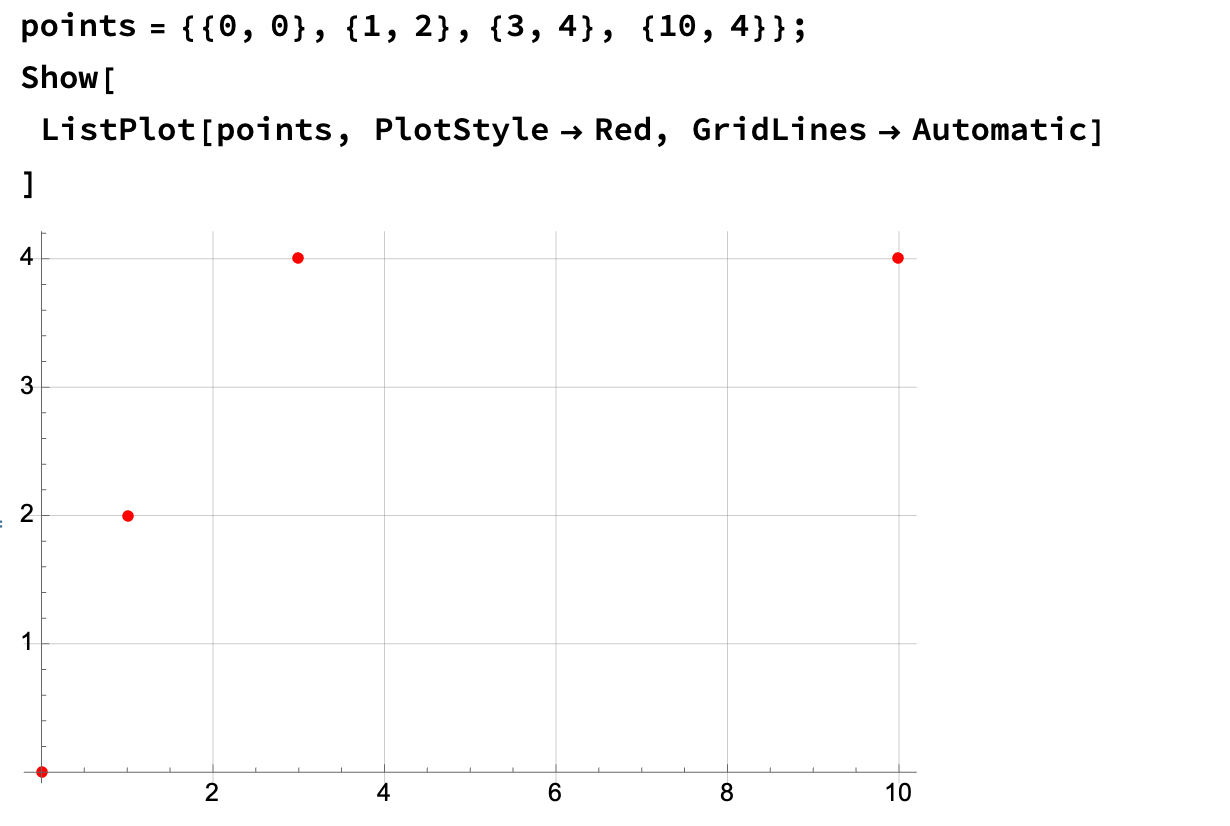
\includegraphics[width=0.7\textwidth]{images/lagrange_example1.png}
\end{figure}

Now, let's use the \texttt{Langrage} module that we have written, and create 
a Lagrange polynomial interpolating the above-mentioned set of points.
\begin{figure}[H]
\centering
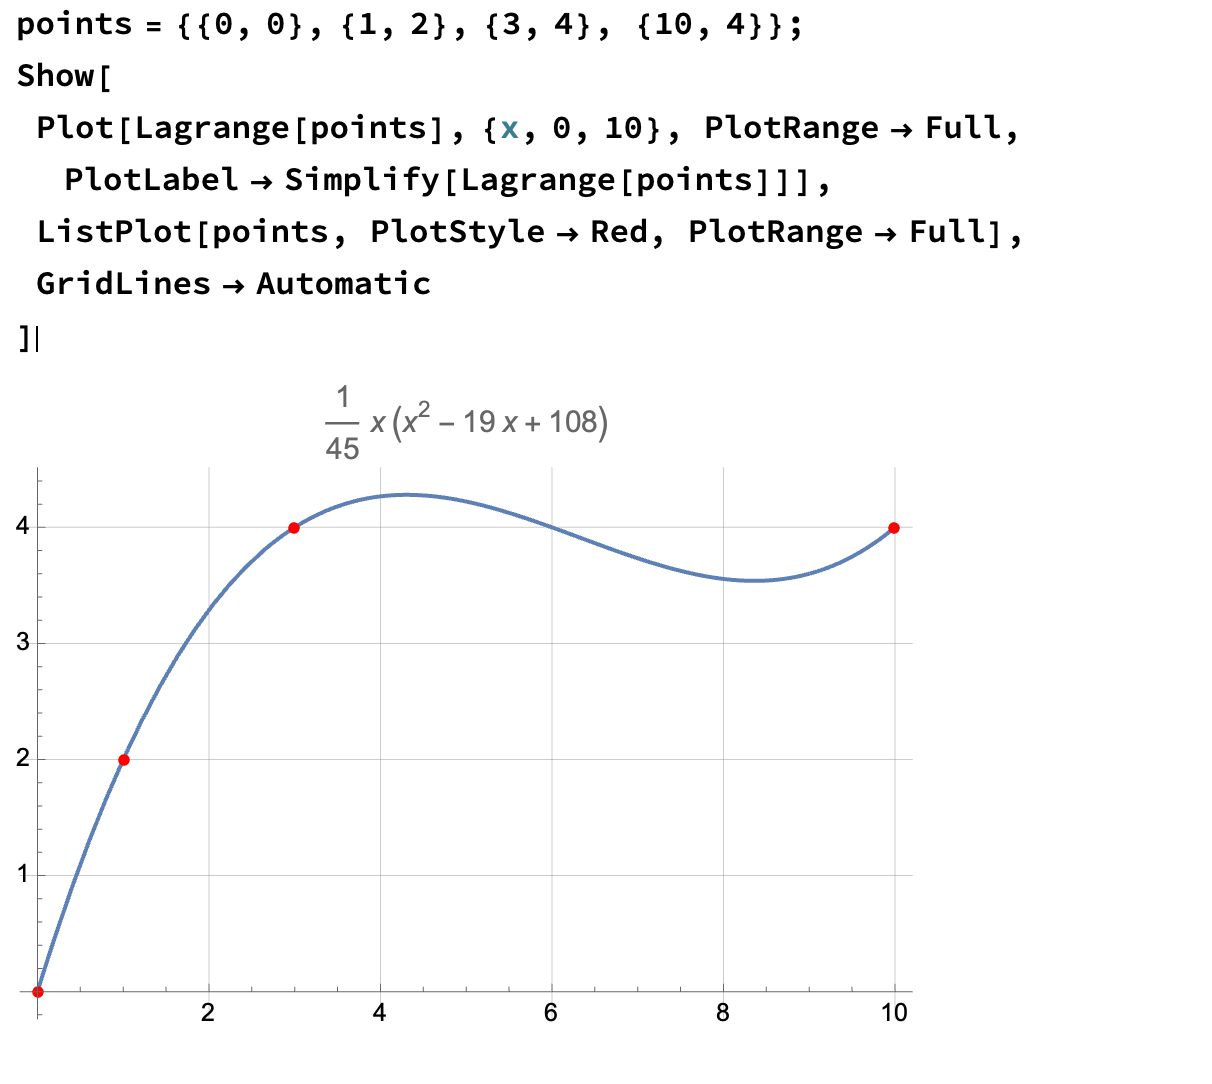
\includegraphics[width=0.7\textwidth]{images/lagrange_example2.png}
\end{figure}

As was previously mentioned, the Lagrange interpolating polynomial is a 
polynomial the of lowest degree that interpolates a given set of data. Thus,
feeding two points into our module will yield a linear function that 
interpolates these points.
\begin{figure}[H]
\centering
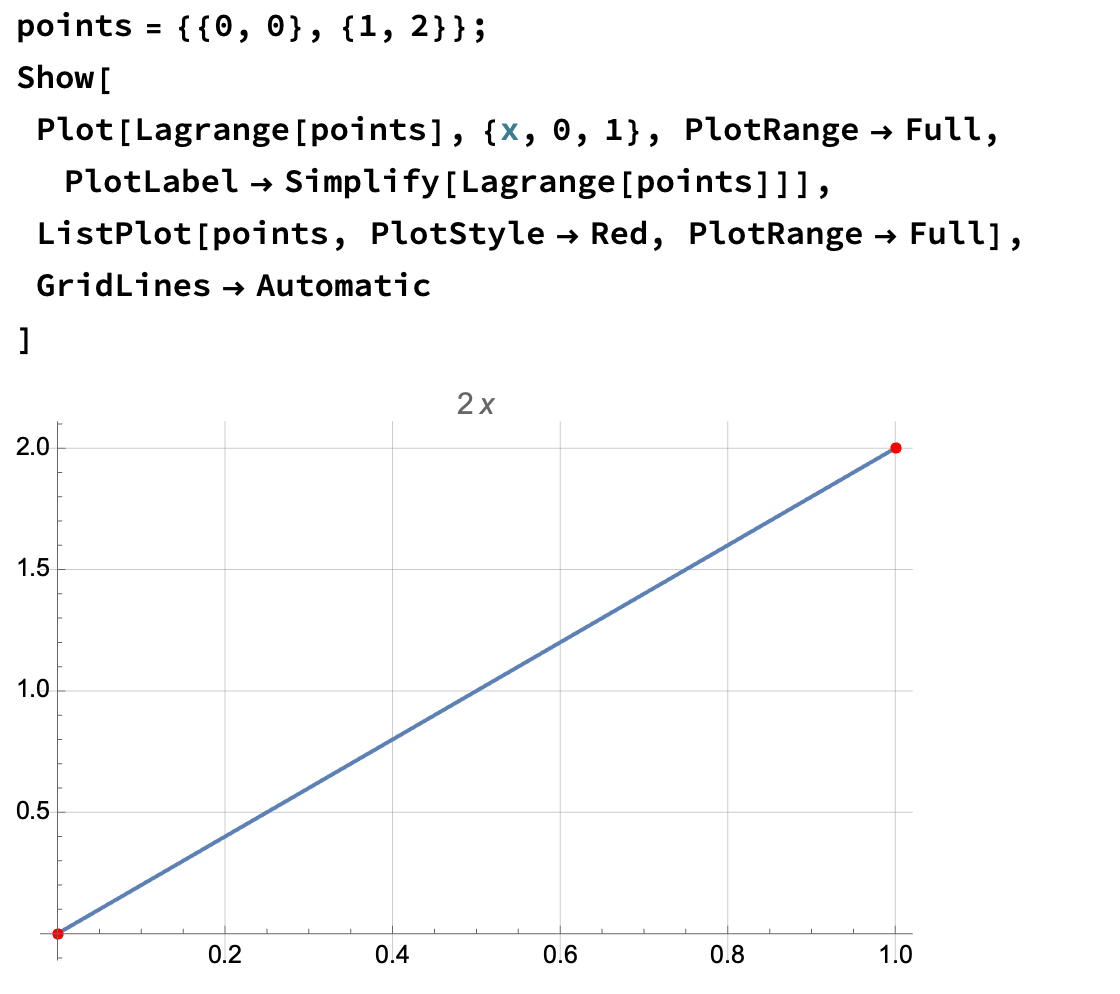
\includegraphics[width=0.7\textwidth]{images/lagrange_example3.png}
\end{figure}

Similarly, three points will yield a quadratic (parabolic) function.
\begin{figure}[H]
\centering
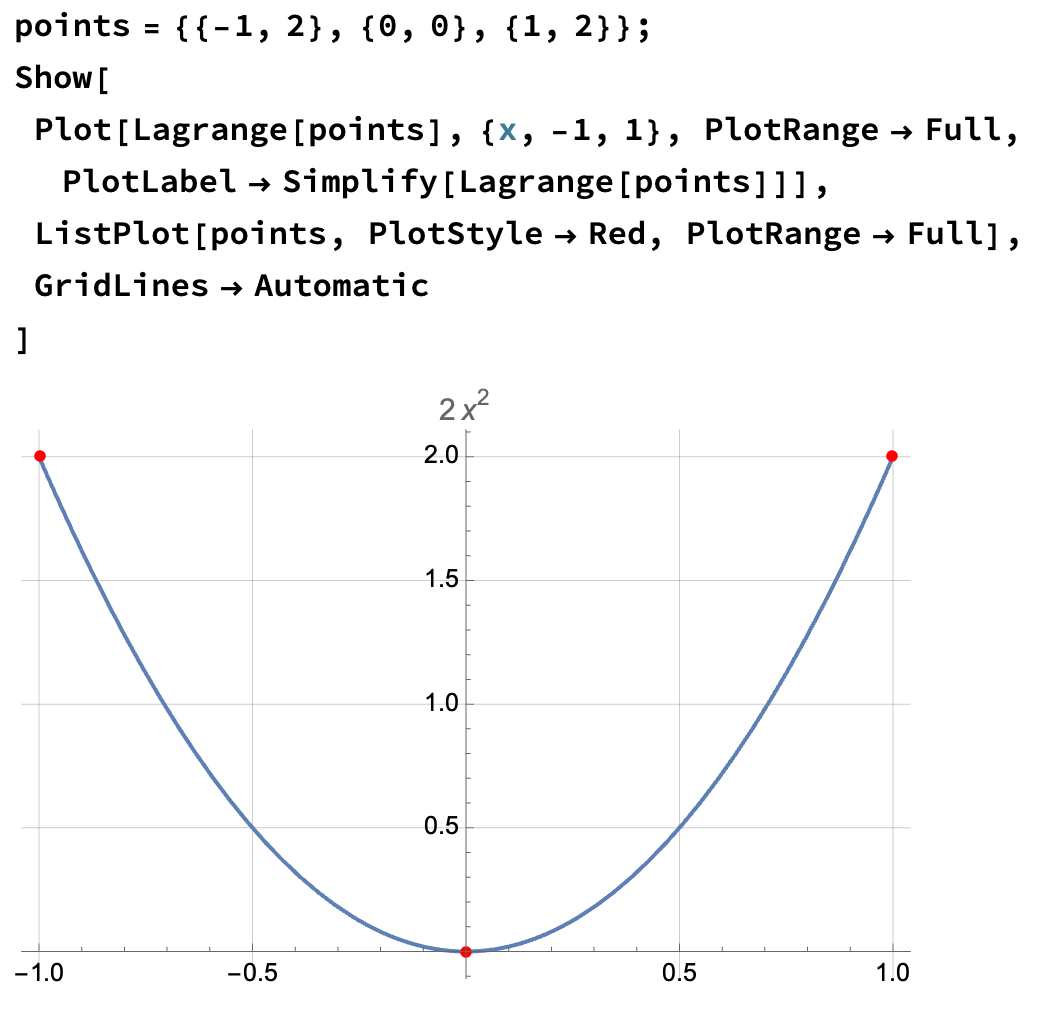
\includegraphics[width=0.7\textwidth]{images/lagrange_example4.png}
\end{figure}


\subsection{Pros and cons of using Lagrange polynomials for approximation}

\textsc{Pros}
\begin{itemize}
	\item The function goes exactly through the set of points given as the input,
	\item The formula is quite easy to understand, as I tried to demonstrate in
		section 2.2,
	\item Even when the points are not evenly spaced, it can be used to find the 
		interpolating function.
\end{itemize}

\textsc{Cons}
\begin{itemize}
	\item As new points are added to the dataset, the function quickly becomes
		computationally complex,
	\item Unsuitable for cases where the general shape of the function is known
		e.g. when we know the function we are looking for should be roughly
		logarithmic, it's better to use the least-squares function approximation
\end{itemize}

% TODO:
\section{Fourier series}

\section{The least squares method}
\textbf{The least squares fitting method} is a widely used technique in statistical
analysis and regression modeling. It aims to find the best-fitting line or curve
for a set of data points by minimizing the sum of the squares of the
vertical distances (residuals) between the data points in the set and the
corresponding points on the fitted line or curve. 

\subsection{How to fit a line to a set of points?}
When trying to find the line of best fit for a given data set, we will be using
a linear function \( f(x) = ax + b \)  as a basis for the least squares method.

Let's imagine that we are looking for a line \( f(x) = ax + b \) that best fits 
a set of points : \( \{(x_1,y_1), (x_2,y_2),\ldots,(x_n,y_n)\} \). 
In order to measure how much the line deviates from the points, we can introduce
residuals (vertical distances) \( \xi_i = | f(x_i) - y_i |  \). 

The problem of finding that line boils down to minimizing the sum of the 
squares of the residuals.

\subsection{Geometric interpretation}
Let's imagine that we are looking for a line \( f(x) = ax + b \) that best fits 
a set of points : \( \{(0,1), (3,1), (4,5)\} \). In order to find this line,
we have to find a formula for the squares of the residuals and minimize it.

Geometrically, it presents as follows:
\begin{center}
	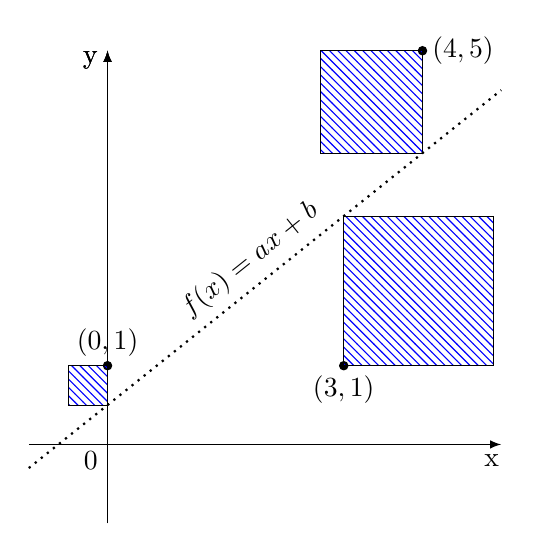
\begin{tikzpicture}
% Axes
\draw[-latex] (-1,0) -- (5,0) node [pos=0.98, below] {x};    
\draw[-latex] (0,-1) -- (0,5) node [pos=0.98, left] {y};    

\draw (0,0.1)--(0,-0.2) node [left] {0};

% Points
\filldraw (0,1) circle[radius=1.5pt] node [above] {\((0,1)\)};
\filldraw (3,1) circle[radius=1.5pt] node [below] {\((3,1)\)};
\filldraw (4,5) circle[radius=1.5pt] node [right] {\((4,5)\)};

\draw[-latex] (0,-1) -- (0,5) node [pos=0.98, left] {y};
\draw[-latex] (0,-1) -- (0,5) node [pos=0.98, left] {y};

% squares
\draw[pattern=north west lines, pattern color=blue] (0,1) rectangle (-0.5,0.5);
\draw[pattern=north west lines, pattern color=blue] (3,1) rectangle (4.9,2.9);
\draw[pattern=north west lines, pattern color=blue] (4,5) rectangle (2.7,3.7);

% Line of best fit
\draw [dotted, thick] (-1, -0.3) -- (5,4.5) node[midway,above,sloped] (line_annotation) {$f(x)=ax+b$};
\end{tikzpicture}
\end{center}
The distance in the vertical direction between the point and the line is the 
residual \( \xi \) of that point. The squares represent \( \xi^2 \) -- which is
the parameter that we're trying to minimize.

\subsection{The optimization problem}
The parameter that we're trying to minimize (optimize) is the sum of the squares
of the residuals \( R^2 = \sum_{i=1}^{n} \xi_i^2 \) with respect to the parameters of 
the linear function \( a, b \).

\[
	R^2 = \sum_{i=1}^{n} \xi_i^2 = \sum_{i=1}^{n} \left[ y_i - (ax_i + b) \right]^2
\]

The condition for \( R^2 \) to be a minimum is that the derivatives of \( R^2 \)
with respect to \( a \) and \( b \) are both equal to zero.
\begin{equation*}
	\begin{aligned}
		\frac{\partial R^2}{\partial a} & = -2\sum_{i=1}^n x_i[y_i-(ax_i+b)] = 0 \\
		\frac{\partial R^2}{\partial b} & = -2\sum_{i=1}^n [y_i-(ax_i+b)] = 0 \\
	\end{aligned}
\end{equation*}

Which we can quickly verify with Wolfram Mathematica
\begin{figure}[H]
\centering
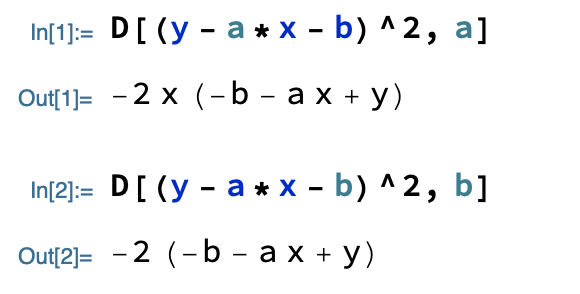
\includegraphics[width=0.5\textwidth]{images/least_squares_derivatives.png}
\end{figure}

This leads to the equations
\begin{equation*}
	\begin{aligned}
		na + b \sum_{i=1}^{n} x_i	= & \sum_{i=1}^{n} y_i \\
		a \sum_{i=1}^{n} x_i + b \sum_{i=1}^{n} x_i^2 = & \sum_{i=1}^{n} x_i y_i
	\end{aligned}
\end{equation*}

Which ultimately leads to the solution for \( a \) and \( b \)
\begin{equation*}
	\begin{aligned}
	a & = \frac{\sum_{i=1}^{n}y_i\sum_{i=1}^{n}x_i^2-\sum_{i=1}^{n}x_i\sum_{i=1}^{n}x_iy_i}{n\sum_{i=1}^{n}x_i^2-(\sum_{i=1}^{n}x_i)^2} \\
	b & = \frac{n\sum_{i=1}^{n}x_iy_i-\sum_{i=1}^{n}x_i\sum_{i=1}^{n}y_i}{n\sum_{i=1}^{n}x_i^2-(\sum_{i=1}^{n}x_i)^2}
	\end{aligned}
\end{equation*}


\section{Summary}

\section*{Enclosures} 
\begin{itemize}
	\item File with the program (\texttt{Pietrasik\_Lewandowicz\_Hankus.nb})
\end{itemize}


\end{document}
